\documentclass[a4paper]{article}

%\usepackage{fullpage} % Package to use full page
\usepackage{parskip} % Package to tweak paragraph skipping
\usepackage{tikz} % Package for drawing
\usepackage{amsmath}
\usepackage{hyperref}
\usepackage[T1]{fontenc}
\usepackage[utf8]{inputenc}
\usepackage[french]{babel}
\usepackage{wrapfig}

\title{Semaine du 06/08}
\author{Reda YAHOU}
\date{\today}

\begin{document}

\maketitle

\section*{Introduction}

Ce document a pour but de résumer le travail qui a été réalisé durant la semaine du 07/08. Ce papier a pour but de proposer un algorithme afin de modéliser la trajectoire et la stabilité des fusées pour le cas bi-étagées.\\




\begin{figure}[!htbp]
\begin{center}
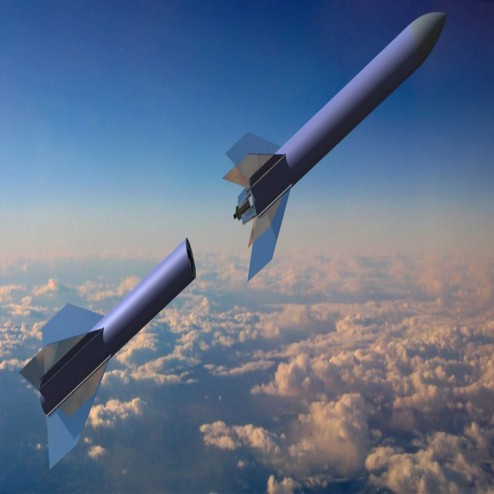
\includegraphics[width=6cm]{pictures/complet-1024x494.jpg} 
\end{center}
\caption{Fusée bi-étage.}
\end{figure}





\section{Vol des fusées bi-étagée}

L'interface Pégase ne réalise les calculs que pour les fusées mono étagées. Le cas des fusées multi-étagée est un peu différent dans la mesure ou il fait entrer d'autres paramètres en jeu : \\

\begin{itemize}
\item La fusée se sépare de ses étages à un moment donnée, entrainant un changement de masse et de géométrie.
\item Il faut par la suite considérer le vol de chaque étage de la fusée indépendamment.
\end{itemize}

En résumé le vol se déroule en trois grandes phases : 

\begin{enumerate}

\item Vol en configuration bi-étage entre $t_{0}$\footnote{instant initial} et $t_{1}$\footnote{instant de séparation},
\item Vol du premier étage seul indépendamment,
\item Vol du deuxième étage seul indépendamment

\end{enumerate}



Les changements de masse et de géométrie vont avoir un impact direct sur les forces mise en jeu et donc sur le schéma numérique modélisant la trajectoire.


\section{Stabilité et trajectoire}


\begin{wrapfigure}[8]{r}{2cm}

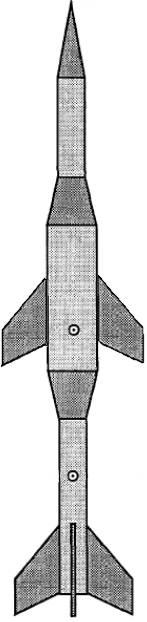
\includegraphics[width=3cm]{pictures/bietage.png}
\end{wrapfigure}

Dans le cas bi-étagé, le vol se réalisant en 3 configurations il faut considérer : la
stabilité de la fusée dans sa totalité avec tout ses éléments (phase bi-étagée), puis la phase post-séparation ou
chaque étage effectue sa trajectoire indépendamment.\\

Il faut calculer la stabilité du première étage dont 
la géométrie est différente (absence d'ogive, ailerons etc.)
et de même pour\\
 l'étage 2
qui se retrouve sans les éléments
géométriques qui \\
constituaient l'étage 1. Les calculs utilisentla méthode de\\
Barrowman permettant de calculer la position du \\
Centre de poussée aérodynamique (Cpa) ainsi que le \\
gradient de portance $C_{N}\alpha$ basé justement sur la géométrie\\
de la fusée et du type d'éléments qui la constituent : \\
présence d'ailerons ou non, présence de jupes ou de rétreints etc.\\


Pour la partie trajectoire, il faut prendre en considération les\\
changements qui occurrent durant la séparation de la fusée

\begin{itemize}
\item changements de masses modifiant les forces et la trajectoire
\item changement de débit massique pour chaque étage
\item changement de géométrie (résistance à l'air)
\end{itemize}

Après la séparation à t=$t_{1}$ le premier étage continue sa trajectoire \\de manière classique (voir rapport 1) alors que l'étage 2 va se rallumer\\ à un temps $t_{2}$, résultant en une seconde phase propulsée pour repartir \\sur une phase \\balistique à un instant $t_{3}$. En résumé, la trajectoire du second étage\\ indépendant peut se synthétiser comme tel : \\

  


\begin{itemize}
\item À t=$t_{1}$ séparation et poursuite de la phase balistique.
\item À t=$t_{2}$ ré-allumage de l'étage et nouvelle phase propulsée.
\item À t=$t_{3}$ épuisement de l'ergol et nouvelle phase balistique puis trajectoire classique.

\end{itemize}


\newpage 

\section{Schéma numérique}

Au vue des informations abordés dans le paragraphe précédent, voici un résumé des étapes de calculs modélisant le vol bi-étagé :

\begin{verbatim}

\\Données : M_0,i, M_1,i, M_2,i -> m_total, m_étage 1 et m_étage 2 (à ti)
dm_1, dm_2 \\ débit massique de l'étage 1 (resp. 2)


****Test de stabilité ******************************************

-> Validation des critères de stabilités pour la fusée bi-étage et
\\pour chaque étage indépendamment :

\\marge statique entre 1.5 est 7.
\\C_N_a compris entre 15 et 30.
\\produit de ces deux paramètres entre 30 et 100.
\\ksi entre 0.05 et 0.2


****Calcul de trajectoire ***************************************

-> Phase propulsée avant t1, cas bi-étage

M_2,i = M_2,0		  \\m_étage 2 ne varie pas pendant cette étape	
M_0,i = M0 - dm_1.ti  \\Màj masse_total avec débit dm_1

R_i  = (1/2)rho_i.C_Ai.S(V_i-1)^2  \\ Résistance de l'air
P_i  = poussée calculée par méthode getloidePoussée1() assosciée à étage 1

	\\Calcul par intégration numérique classiques

	Gamma_xi = (P_i - R_i)/M_0,i . cos(theta_i-1)		//accélérations
	Gamma_zi = (P_i - R_i)/M_0,i .sin(theta_i-1) - g

	X_i = X_i-1 + (V_xi-1).dt_i +(1/2)(Gamma_xi).(dt_i)^2	\\selon x
	Z_i = Z_i-1 + (V_zi-1).dt_i +(1/2)(Gamma_zi).(dt_i)^2	\\selon z

	a = tan(theta_i-1) = (V_zi)/(V_xi)
	theta_i = arctan(a)

->Séparation à t = t1

	\\Màj des masses, positions, vitesses
	m_étage 1 = M_1,i - dm(t0+..+t1)
	m_étage 2 = M_2,i= M_2,0	
	theta_i,1 = theta_i,2 = theta_i
	Vi,1 = Vi,2 = Vi
	Xi,1 = X,i - dist(cdm0,cdm1); Xi,2 = X,i - dist(cdm0,cdm2)

-> Trajectoire des 2 étages après séparation 

	\\->étage 1 **
	
	\\plus de poussée dans gamma car phase balistique
	R_i,1  = (1/2)rho_i,1.C_Ai,1.S(V_i-1,1)^2  \\ Résistance de l'air

	\\Calcul par intégration numérique classiques

	Gamma_xi,1 = (- R__i,1)/m_étage 1 . cos(theta_i-1)		//accélérations
	Gamma_zi,1 = (- R_i,1)/m_étage 1 .sin(theta_i-1) - g

	X_i,1 = X_i-1,1 + (V_xi-1,1).dt_i +(1/2)(Gamma_xi,1).(dt_i)^2	\\selon x
	Z_i,1 = Z_i-1,1 + (V_zi-1,1).dt_i +(1/2)(Gamma_zi,1).(dt_i)^2	\\selon z

	a1 = tan(theta_i-1,1) = (V_zi,1)/(V_xi,1)
	theta_i,1 = arctan(a1)

	\\->étage 2 **
	
		\\\\ Entre t1 et t2 = phase balistique

	\\plus de poussée dans gamma car phase balistique
	R_i,2  = (1/2)rho_i,2.C_Ai,2.S(V_i-1,2)^2  \\ Résistance de l'air

	\\Calcul par intégration numérique classiques

	Gamma_xi,2 = (- R_i,2)/m_étage 2 . cos(theta_i-1)		//accélérations
	Gamma_zi,2 = (- R_i,2)/m_étage 2.sin(theta_i-1) - g
	
	
		X_i,2 = X_i-1,2 + (V_xi-1,2).dt_i +(1/2)(Gamma_xi,2).(dt_i)^2	\\selon x
		Z_i,2 = Z_i-1,2 + (V_zi-1,2).dt_i +(1/2)(Gamma_zi,2).(dt_i)^2	\\selon z

		a2=tan(theta_i-1,2) = (V_zi,2)/(V_xi,2)
		theta_i,2 = arctan(a2)

		\\\\Entre t2 et t3 = phase propulsée i.e ré-allumage
		
		m_étage 2 = M_2,i = M2,0 - dm_2.ti
		P_i,2  = poussée calculée par méthode getloidePoussé21() assosciée à étage 2
		\\reprise de pousée
		
		X_i,2 = X_i-1,2 + (V_xi-1,2).dt_i +(1/2)(Gamma_xi,2).(dt_i)^2	\\selon x
		Z_i,2 = Z_i-1,2 + (V_zi-1,2).dt_i +(1/2)(Gamma_zi,2).(dt_i)^2	\\selon z
		
		\\\\Après t3
		\\phase balistique donc plus de poussée dans le calcul de gamma
		
		X_i,2 = X_i-1,2 + (V_xi-1,2).dt_i +(1/2)(Gamma_xi,2).(dt_i)^2	\\selon x
		Z_i,2 = Z_i-1,2 + (V_zi-1,2).dt_i +(1/2)(Gamma_zi,2).(dt_i)^2	\\selon z
*************************************************************************


\end{verbatim}


Pour le reste des phases de vol\footnote{On peut considérer pendant le vol bi-étagée lors de la phase propulsée l'existence d'une rampe surélevée. On peut voir les modifications à apporter dans l'algorithme dans le rapport 1.} (ouverture du parachute), il suffit simplement d'appliquer le même algorithme décrit dans le paragraphe précédent : 

\begin{verbatim}
P = R   V = Cste = V_l 
M.g = (1/2).rho.S_para.C_x_para.V_l
V_l = (2.M.g/(rho.S_par.C_x_par))^(1/2)

\\avec V_l = vitesse limite

\end{verbatim}





\section{Conclusions}

La prochaine étape du projet sera l'écriture de cet algorithme en JAVA, l'incorporer à la plateforme Pégase, réaliser des tests et corriger les éventuelles erreurs et/ou ajouter les détails qui pourraient manquer pour modéliser rigoureusement le vol bi-étage.

%\bibliographystyle{plain}
%\bibliography{bibliography.bib}
\end{document}
